\documentclass[12pt]{beamer}


% INCLUDE GRAPHICS
\usepackage{graphicx}

% TABLES
\newcommand{\ra}[1]{\renewcommand{\arraystretch}{#1}} % spaces in tables
\usepackage{booktabs}   % Allows the use of \toprule, \midrule and \bottomrule in tables for horizontal lines


% FONTS
% PdfLatex
% \usepackage[T1]{fontenc}
% \usepackage{pgf}
% \logo{\pgfputat{\pgfxy(-1,-0.435)}{\pgfbox[center,base]{
\includegraphics[width=1.2cm,natwidth=610,natheight=642]{KUNATLogo.pdf}}}}

% FONTS
% xelatex
\usepackage{fontspec}
% \setsansfont{TeX Gyre Heros}
% \setsansfont{TeX Gyre Heros Cn}
\setsansfont{Helvetica Neue}

% Use serif for Math environments
\usefonttheme[onlymath]{serif}


% CODE
\usepackage{listings} % Code block (source code) \begin{lstlisting}
\lstset{
    language=Python,                        % Code langugage
    commentstyle=\color{gray},              % Comments font
    basicstyle=\small\ttfamily,             % Code font, Examples: \footnotesize, \ttfamily
    keywordstyle=\bfseries\color{blue},
    stringstyle=\color{orange},
    numbers=left,                           % Line nums position
    numberstyle=\tiny,                      % Line-numbers fonts
    stepnumber=1,                           % Step between two line-numbers
    numbersep=5pt,                          % How far are line-numbers from code
    numbers=none,
    frame=single,                             % A frame around the code
    tabsize=4,                              % Default tab size
    captionpos=b,                           % Caption-position = bottom
    breaklines=true,                        % Automatic line breaking?
    breakatwhitespace=false,                % Automatic breaks only at whitespace?
    showspaces=false,                       % Dont make spaces visible
    showstringspaces=false,                 % Dont make spaces visible in strings
    showtabs=false,                         % Dont make tabls visible
    belowskip=8pt,
    morekeywords={range, xrange},
    backgroundcolor=\color{white}
    % emph={[2]root,base}
    % morekeywords={one,two,three,four,five,six,seven,eight,
}
\newcommand{\code}[1]{{\small\ttfamily #1}} % \code{inline code}

%
% COLORS
%
\definecolor{kugreen}{RGB}{50,93,61}

\definecolor{orange}{RGB}{255,127,0}
\definecolor{green}{RGB}{0,153,51}
\definecolor{blue}{RGB}{3,115,187}
\definecolor{red}{RGB}{221,17,68}
\definecolor{gray}{RGB}{55,55,55}
\definecolor{black}{RGB}{0,0,0}

\definecolor{offwhite}{RGB}{249,242,215}
\definecolor{foreground}{RGB}{23,23,23}
\definecolor{background}{RGB}{255,255,255}
\definecolor{subtitle}{RGB}{102,255,204}
\definecolor{hilight}{RGB}{102,255,204}
\definecolor{vhilight}{RGB}{255,111,207}
\definecolor{lolight}{RGB}{155,155,155}


%
% BEAMER STYLE COLORS
%
\setbeamercolor{titlelike}{fg=black}
\setbeamercolor{subtitle}{fg=blue}
\setbeamercolor{institute}{fg=gray}
\setbeamercolor{normal text}{fg=foreground,bg=background}
\setbeamercolor{item}{fg=foreground} % color of bullets
\setbeamercolor{subitem}{fg=gray}
\setbeamercolor{itemize/enumerate subbody}{fg=gray}

% \setbeamertemplate{itemize item}{\tiny $\bullet$}
% \setbeamertemplate{itemize subitem}{{\textendash}}

\setbeamerfont{itemize/enumerate subbody}{size=\footnotesize}
\setbeamerfont{itemize/enumerate subitem}{size=\footnotesize}

\setbeamerfont{footnote}{size=\tiny}

\setbeamersize{text margin left=10pt}
\setbeamersize{text margin right=10pt}
\setbeamersize{sidebar width right=0pt}
\setbeamersize{sidebar width left=0pt}

%
% REMOVES THE NAVIGATION BAR
%
\beamertemplatenavigationsymbolsempty


% BEAMER TEMPLATES


%
% BEAMER BACKGROUND
%
\usebackgroundtemplate{

    \rule{0pt}{0.97\paperheight}%
    \hspace*{1.15\paperwidth}%
    \makebox[0pt][r]{%
        
\includegraphics[width=100pt,natwidth=610,natheight=642]{KUNATLogo.pdf}
    }

}


%
% BEAMER HEADLINE
%
\setbeamertemplate{headline}{}


%
% BEAMER TITLE
%
\setbeamertemplate{frametitle}
{
    \begin{centering}
    \insertframetitle\par
    \end{centering}
}


%
% BEAMER FOOTER
%
\setbeamertemplate{footline}[text line]
{%
    \vbox{%
        \insertvrule{0.5pt}{kugreen}

        \vspace{2pt}

        \strut{
        % \rmfamily\itshape
        \expandafter\insertshorttitle
        \expandafter\insertauthor
        \insertshortinstitute
        }
        \hfill\strut{
        }
        \hfill\strut{
            \insertframenumber\,/\,\inserttotalframenumber
        }

        \vspace{1pt}
    }
}


%
% TITLE PAGE
%
% \setbeamertemplate{title page}
% {
%     % Remove beamer background
%     \setbeamertemplate{background}{}
% 
%     \begin{beamercolorbox}[center]{beamer color}
% 
%         {
%             \huge
%             \color{kugreen}
%             \inserttitle
%         }
%         \bigskip
%         \bigskip
% 
%         % 
\includegraphics[width=2cm]{KUNATLogo}
% 
%         \bigskip
%         {
%             \bf
%             \rmfamily
%             {\large \insertauthor}
%         }
% 
%         \smallskip
%         {
%             \rmfamily
%             \footnotesize
%             \insertinstitute
%         }
% 
%         {
%             \rmfamily
%             \footnotesize
%             \insertdate
%         }
% 
%     \end{beamercolorbox}
% 
%     % Do not count the title page
%     \addtocounter{framenumber}{-1}
% }


\title[]{New Computational Methods\\ for Drug Design}
% \subtitle[]{Fast quantum mechanics for bio-chemistry}
\institute[, University of Copenhagen]{Department of Chemistry \\ University of Copenhagen}
\author[J. C. Kromann]{Jimmy Charnley Kromann}
\date{
    \href{http://jimmy.charnley.dk}{\tt \scriptsize jimmy.charnley.dk}
    \\[-4pt]
    \href{http://github.com/charnley}{\tt \scriptsize github.com/charnley}
}


\begin{document}

{
\usebackgroundtemplate{}
\frame[plain]{\titlepage}
}

%%%%%%%%%%%%%%%%%%%%%%%%%%%%%%%%%%%%%%%%%%%%%%%%%%%%%%%%%%%%%%%%%%%%%%
%% BEGIN FRAMES
%%%%%%%%%%%%%%%%%%%%%%%%%%%%%%%%%%%%%%%%%%%%%%%%%%%%%%%%%%%%%%%%%%%%%%

\begin{frame}

    \frametitle{What is the problem?}

    Proteins are sooo big

\end{frame}


\begin{frame}

    \frametitle{Available tools}

    current methods, much slow

\end{frame}


\begin{frame}

    \frametitle{What is the solution?}

    MM, SQM, FMO

\end{frame}


\frame
{
    \frametitle{Good Artists Copy; Great Artists Steal}

    \centering

    \begin{align*}
        { \overbrace{E(\mathrm{PM6\text{-}D3H+})}^\text{Kromann et al} } =
        { \overbrace{ E(\mathrm{PM6}) }^\text{Stewart} } +
        { \overbrace{ E(\mathrm{D3}) }^\text{Grimme et al} } +
        { \overbrace{ E(\mathrm{H+}) }^\text{Korth} }
    \end{align*}

    % $$
    % E(\mathrm{PM6\text{-}D3H+}) =
    % E(\mathrm{PM6}) +
    % E(\mathrm{D3}) +
    % E(\mathrm{H+})
    % $$

    \bigskip

    % {\scriptsize
    %     Kromann {\em et al} ({\bf 2014}) PeerJ 2:e449 http://dx.doi.org/10.7717/peerj.449
    % }

    {\scriptsize
        {\bf J. C. Kromann}, A. S. Christensen, C. Steinmann, M. Korth and J. H. Jensen\\
        PeerJ
        {\bf 2014}
        2:e449
        {10.7717/peerj.449}
    }

    % title = {{A third-generation dispersion and third-generation hydrogen bondingcorrected PM6 method: PM6-D3H+}},

    \bigskip

    \bigskip

    \bigskip

    HF-3c/FMO Interface

    \bigskip

    {\scriptsize
        {\bf J. C. Kromann} and J. H. Jensen\\
        Unpublished
    }

}


\frame
{
    \frametitle{Yet another fitted method}

    \begin{columns}[c]
        \column{0.7\linewidth}

            \centering

            {\small Interaction energies [kcal/mol]}

            \bigskip
            {

            \footnotesize

            \begin{tabular}{ @{} l r r r r @{} }
                \ra{1.3}
                & {\color{red}PM6}
                & {\color{blue}PM6-DH+}
                & {\color{kugreen}PM6-D3H+}
                & HF-3c \\
                \midrule
                \multicolumn{5}{c}{\small All Complexes} \\
                \midrule

                RMSD & {\color{red}3.35} & {\color{blue}0.80} & {\color{kugreen}0.83} & {0.54} \\
                 MAD & {\color{red}2.85} & {\color{blue}0.61} & {\color{kugreen}0.60} & {0.39} \\

                && \\
                \multicolumn{5}{c}{ \small Dispersion Complexes} \\
                \midrule

                RMSD & {\color{red}3.15} & {\color{blue}0.49} & {\color{kugreen}0.48} & {0.58} \\
                 MAD & {\color{red}2.79} & {\color{blue}0.42} & {\color{kugreen}0.36} & {0.43} \\

                && \\
                \multicolumn{5}{c}{ \small Hydrogen-bond Complexes} \\
                \midrule

                RMSD & {\color{red}4.29} & {\color{blue}0.98} & {\color{kugreen}1.11} & {0.63} \\
                 MAD & {\color{red}3.65} & {\color{blue}0.80} & {\color{kugreen}0.92} & {0.51} \\

            \end{tabular}

            }


        \column{0.35\linewidth}

            {

            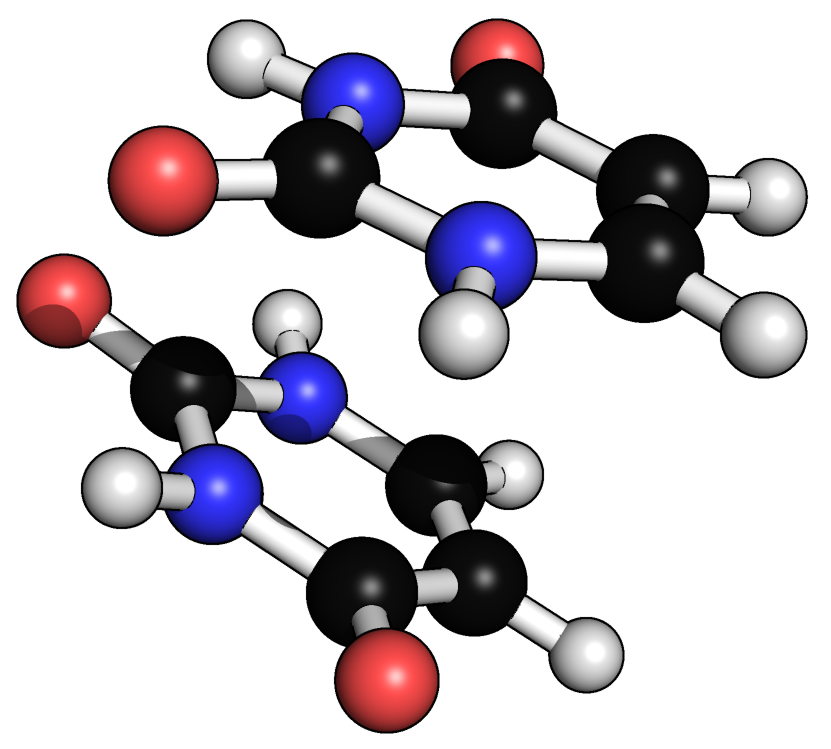
\includegraphics[width=1.0\linewidth]{figures/s22_13.png}

            }


    \end{columns}

}



\begin{frame}
    \frametitle{Structure refinement of small proteins}
    
    \begin{center}
    PM6-D3H+
    \end{center}

    \begin{columns}[t]
        \column{0.5\linewidth}

            {\bf 1L2Y } 304 atoms\\
            RMSD 0.83 \AA

            \bigskip

            \includegraphics[width=1.0\linewidth]{figures/1L2Y_pm6-d3h+}

        \column{0.4\linewidth}


            {\bf 1UAO } 138 atoms\\
            RMSD: 0.93 \AA

            \bigskip

            \includegraphics[width=0.8\linewidth]{figures/1UAO_pm6-d3h+}



    \end{columns}

\end{frame}



\begin{frame}

    \frametitle{Refining Proteins Structures}

    % \begin{tabular}{@{} l l r r r r r r r r r @{} }
    %     \multicolumn{2}{c}{} &
    %     \multicolumn{4}{c}{PM6-DH+} &
    %     \multicolumn{4}{c}{PM6-D3H+}\\
    %     \cmidrule(l){3-6} \cmidrule(l){7-10}
    %     
    %     System & PDB & RMSD [\AA ] & Time [h] & Steps & $N_i$ & RMSD [\AA ] & Time [h] & Steps & $N_i$ \\
    %     
    %     \midrule
    %     
    %     Chignolin & 1UAO & 0.90 & 0.1 & 739 & 4 & 0.98 & 0.2 & 204 & 0 (0) \\
    %     Trp-Cage  & 1L2Y & 1.89 & 1.1 & 1774 & 2 & 1.61 & 5.4 & 481 & 2 (0)\\


    %     % SOLVENT

    %     \midrule
    %     
    %     Chignolin & 1UAO & 1.14 & 0.1 & 941 & 5 & 0.56 & 0.6 & 128 & 3 (0) \\
    %     Trp-Cage  & 1L2Y & 1.23 & 0.6 & 882 & 12 & 0.83 & 5.2 & 174 & 2 (0) \\
    %     
    %     \midrule
    %     
    % \end{tabular}


    % Number of imaginary frequencies for OPTTOL = 5 × 10−4 (1 × 10−4 ) aus.

    \begin{columns}

        \column{0.7\linewidth}

        \centering

        \begin{tabular}{@{} l r r r r r @{} }

            PDB & RMSD [\AA] & Time [h] & Steps & $N_i$\\

            \midrule

            &&\\

            \multicolumn{5}{c}{ \small PM6-DH+} \\

            \midrule

            % 1UAO & 0.90 & 0.1 & 739 & 4 \\
            % 1L2Y & 1.89 & 1.1 & 1774 & 2 \\

            1UAO & 1.14 & 0.1 & 941 & 5 \\
            1L2Y & 1.23 & 0.6 & 882 & 12 \\

            &&\\

            \multicolumn{5}{c}{ \small PM6-D3H+} \\

            \midrule

            1UAO & 0.56 & 0.6 & 128 & 0 \\
            1L2Y & 0.83 & 5.2 & 174 & 0 \\
            
            &&\\

            \multicolumn{5}{c}{ \small HF-3c/FMO} \\

            \midrule

            1UAO & 0.83 & 27.9$^b$ & 186 &  n/a \\


        \end{tabular}


        \column{0.4\linewidth}

            \includegraphics[width=0.8\textwidth]{figures/1L2Y.png} \\

            \bigskip

            \bigskip

            {
            \scriptsize

            1UAO: 138 atoms\newline
            1L2Y: 304 atoms\\

            \bigskip

            Ref: FMO2-RHF-D3/\newline
            6-31G(d)/PCM 

            }

            \bigskip

            {\scriptsize
                $b$ 8 cores
            }


    \end{columns}

\end{frame}






\begin{frame}
    \frametitle{Further development}

    
    \begin{columns}[t]
        \column{0.5\linewidth}

            {\bf Work in progress: }

            \begin{itemize}

                \item Accurate ligand-host docking

                \item Enzyme TS prediction

            \end{itemize}

        \column{0.4\linewidth}

            {\bf Next 3 years: }

            \begin{itemize}

                \item $d$-integrals $\in$ GAMESS

                \item PM6-3c
                \item PM6/FMO

            \end{itemize}

    \end{columns}

\end{frame}


\begin{frame}
    \frametitle{Shameless self-promotion}

    \begin{columns}[t]
        \column{0.45\linewidth}


            \begin{itemize}

                \item Molecule Calculator (molcalc.org)

            \end{itemize}

            {\scriptsize
                J. H. Jensen and {\bf J. C. Kromann}\\
                J. Chem. Edu.
                {\bf 2013}
                90(8), 1093-1095
                10.1021/ed400164n

                % (2013). The Molecule Calculator: A Web Application for Fast Quantum Mechanics-Based Estimation of Molecular Properties. Journal of Chemical Education, 90(8), 1093-1095.
            }


        \column{0.5\linewidth}

            \begin{itemize}

                \item github.com/charnley

                \begin{itemize}

                    \item Kabsch RMSD algorithm

                \end{itemize}

                \item github.com/jensengroup

                \begin{itemize}

                    \item molcalc

                    \item H+

                    \item Optimized Protein Structures

                \end{itemize}


            \end{itemize}


    \end{columns}

\end{frame}



\begin{frame}
    \frametitle{Thank you!}

    \begin{columns}[c]

        \column{0.6\linewidth}


            \begin{itemize}

                \item Jan "Yoda" Jensen (supervisor)

                \item Martin Korth (collaborator)

                \item Anders Christensen, Casper Steinmann and Lars Bratholm
                    (extreme caffeine boys)

                \item Kurt Mikkelsen, Stephan Sauer and Sten Rettrup
                    (local prof.)

            \end{itemize}

        \column{0.4\linewidth}

            \includegraphics[width=1.0\linewidth]{figures/larsandanders.jpg}

    \end{columns}


\end{frame}




%%%%%%%%%%%%%%%%%%%%%%%%%%%%%%%%%%%%%%%%%%%%%%%%%%%%%%%%%%%%%%%%%%%%%%
%% END FRAMES
%%%%%%%%%%%%%%%%%%%%%%%%%%%%%%%%%%%%%%%%%%%%%%%%%%%%%%%%%%%%%%%%%%%%%%

\end{document}

